%%%%%%%%%%%%%%%%%%%%%%%%%%%%%%%%%%%%%%%%%%%%%%%%%%%%%%%%%%%%%%%%%%%%
% bare_jrnl.tex
% V1.4b
% 2015/08/26
% by Michael Shell
% see http://www.michaelshell.org/
% for current contact information.                                                                 
%%%%%%%%%%%%%%%%%%%%%%%%%%%%%%%%%%%%%%%%%%%%%%%%%%%%%%%%%%%%%%%%%%%%

%% This is a skeleton file demonstrating the use of IEEEtran.cls
%% (requires IEEEtran.cls version 1.8b or later) with an IEEE
%% journal paper.
%%
%% Support sites:
%% http://www.michaelshell.org/tex/ieeetran/
%% http://www.ctan.org/pkg/ieeetran
%% and
%% http://www.ieee.org/


\documentclass[journal]{IEEEtran}
%
\usepackage{instructivo}  % Commands for multiple choice
\graphicspath{{./}{./fig/}}

\usepackage[natbib=true,style=trad-unsrt,backend=biber]{biblatex}
\addbibresource{literatura.bib}

\usepackage{standalone}
\usepackage[americanresistors,americaninductors,RPvoltages]{circuitikz}

\usepackage{float}
\usepackage{graphicx}
\usepackage{booktabs}
\usepackage{tabularx}
\usepackage{url}
\usepackage{hyperref}


% correct bad hyphenation here
\hyphenation{op-tical net-works semi-conduc-tor}


\begin{document}
%
% paper title
% Titles are generally capitalized except for words such as a, an, and, as,
% at, but, by, for, in, nor, of, on, or, the, to and up, which are usually
% not capitalized unless they are the first or last word of the title.
% Linebreaks \\ can be used within to get better formatting as desired.
% Do not put math or special symbols in the title.
\title{Tarea 1: Circuitos Térmicos y el Convertidor Buck}


\author{Matías~A.~Camacho,~\IEEEmembership{estudiante,~TEC}
        ,~Juan~P.~Elizondo,~\IEEEmembership{estudiante,~TEC}
        ~y~Fernando~J.~Rodriguez,~\IEEEmembership{estudiante,~TEC}
}


% The paper headers
\markboth{Procesamiento Electrónico de Potencia, IS2026}%
{Procesamiento Electrónico de Potencia}


% make the title area
\maketitle


\begin{abstract}
El resumen no debe de exceder de 150 palabras y debe establecer lo que fue hecho, como fue hecho, los resultados principales y su significado. No cite referencias en el resumen. No coloque ecuaciones, símbolos especiales o palabras claves.
\end{abstract}

% Se sugiere no más de cuatro palabras o frases cortas en orden alfabético, separadas por comas, que representen su reporte
\begin{IEEEkeywords}
Convertidor, ganancia, temperatura, eficiencia, potencia.
\end{IEEEkeywords}


%%%%%%%%%%%%%%%%%%%%%%%%%%%%%%%%%%%%%%%%%%%%%%%%%%%%%%%%%%%%%%%%%%%%%%%%%%%%%%%%%%%%%%%%%%%%%%
%%%%%%%%%%%%%%%%%%%%%%%%%%%%%%%%%%%%%%%%%%%%%%%%%%%%%%%%%%%%%%%%%%%%%%%%%%%%%%%%%%%%%%%%%%%%%%
\section{Introducción}

\IEEEPARstart{E}{n} esta sección se describe una introducción que le permita al lector 
identificar aspectos importantes para la comprensión de la lectura del documento, una visión 
relacionada al experimento y a los conocimientos científicos estudiados.


%%%%%%%%%%%%%%%%%%%%%%%%%%%%%%%%%%%%%%%%%%%%%%%%%%%%%%%%%%%%%%%%%%%%%%%%%%%%%%%%%%%%%%%%%%%%%%
%%%%%%%%%%%%%%%%%%%%%%%%%%%%%%%%%%%%%%%%%%%%%%%%%%%%%%%%%%%%%%%%%%%%%%%%%%%%%%%%%%%%%%%%%%%%%%
\section{Fundamentos Teóricos}
Como parte de la ejecución de un buen diseño se presentan los principales fundamentos teóricos 
que sustentan lo realizado en este trabajo.

\subsection{Convertidor Buck}
El convertidor Buck es un convertidor DC-DC reductor que permite obtener un voltaje de salida menor al voltaje de entrada mediante el uso de un interruptor controlado (generalmente un MOSFET), un diodo, un inductor y un capacitor.

Su principio de operación se basa en la conmutación periódica del interruptor, lo cual genera dos estados: conducción y apagado \cite{hart2011power}. En estado de conducción, el inductor almacena energía, mientras que en el estado de apagado, esta energía se transfiere a la carga.

En régimen ideal y en conducción continua, la relación entre el voltaje de salida y el de entrada está dada por:
\begin{equation}
    V_o = D \cdot V_{in}
\end{equation}
donde $D$ es el ciclo de trabajo de la señal de control.

---

\subsection{Pérdidas en semiconductores de potencia}
Las pérdidas en dispositivos semiconductores de potencia determinan su eficiencia y comportamiento térmico. Estas se clasifican principalmente en pérdidas por conducción y por conmutación.

\subsubsection{Perdidas por conducción}
Las pérdidas por conducción ocurren cuando el dispositivo se encuentra en estado ON. En el caso de un MOSFET, estas pérdidas están asociadas a su resistencia de encendido $R_{on}$ y se pueden expresar como:
\begin{equation}
    P_{cond} = I^2 \cdot R_{on}
\end{equation}
donde $I$ es la corriente que circula por el dispositivo \cite{kassakian1991principles}.

\subsubsection{Perdidas por conmutación}
Las pérdidas por conmutación se producen durante los intervalos de encendido y apagado del dispositivo, debido a la superposición de voltaje y corriente. Estas pérdidas dependen de la frecuencia de conmutación y de los tiempos de transición.
\subsubsection{$R_{on}$ y su dependencia con la temperatura}
La resistencia $R_{on}$ de los MOSFETs depende fuertemente de la temperatura de la unión. A medida que la temperatura aumenta, la movilidad de los portadores disminuye, lo que incrementa el valor de $R_{on}$.

Este comportamiento provoca un aumento en las pérdidas por conducción y puede generar un efecto de realimentación térmica si no se controla adecuadamente. Por ello, es fundamental considerar esta dependencia en el diseño térmico del sistema.

\subsection{Modelos térmicos}
    El comportamiento térmico de un semiconductor se puede representar
    mediante un circuito eléctrico equivalente (circuito térmico).

    \setlength{\parskip}{1em}

    \subsubsection{Modelo térmico de Foster}
    Este es un modelo en donde su estructura se basa en una red de pares RC
    en paralelo conectados en serie entre \emph{$T_{j}$} y \emph{$T_{case}$}, según se muestra en la Figura \ref{fig:circuito_foster}. 
    Su singularidad, los nodos de la red no tienen ningún significado físico; es decir, sus elementos RC individuales, 
    ya no representan las secuencias de capas físicas del dispositivo \cite{schutze2008thermal}.

    \begin{figure}[H]
        \centering
        \includestandalone[width=\columnwidth]{circuito_Foster}
        \caption{Topología del modelo Foster}
    \label{fig:circuito_foster}
    \end{figure}

    La impedancia térmica según este modelo, se puede ver en la siguiente ecuación. En donde
    cada par (\emph{$r_{i}$} y \emph{$\tau_{i}$}) se puede obtener de la hoja de datos
    del fabricante. 

    \begin{equation}
        Z_{th,jc}(t) = \sum_{i=1}^{n} r_i \left(1 - e^{-t/\tau_i} \right)
    \end{equation}

    Mientras que la temperatura de juntura se puede calcular como

    \begin{equation}
        T_j(t) = P(t) \cdot Z_{th,jc}(t) + T_{case}(t)
    \end{equation}

    Esta representación también conocida como el circuito de fracción parcial o modelo Pi. 
    Es utilizada en hojas de datos porque los coeficientes pueden extraerse fácilmente de
    la curva de enfriamiento medida del módulo y es de utilidad para realizar cálculos analíticos. 
    No obstante, este es un modelo con un comportamiento de extremo a extremo, lo que quiere decir
    que analiza la caída de temperatura entre la juntura y el encapsulado; por esto, no 
    predice el flujo de calor en la salida y no es posible analizar el modelo del 
    semiconductor conectado a un disipador, ya que genera un error en el momento en el que no 
    se considera el retardo físico real de la potencia al llegar al disipador. 



    \subsubsection{Modelo térmico de Cauer}
    Este modelo es conocido también como el circuito de fracción continua o modelo T. 
    A diferencia del modelo de Foster, este modelo sí refleja la configuración real del 
    semiconductor (capacidades térmicas con resistencias térmicas intermedias) \cite{schutze2008thermal}.

    \setlength{\parskip}{1em}

    Su topología consiste en una red en escalera donde cada nodo intermedio sí
    tiene significado físico y representa una interfaz real entre capas del dispositivo, tal como 
    se muestra en la Figura \ref{fig:circuito_cauer}; de esta manera, los elementos RC individuales 
    pueden ser asignados a las capas individuales del módulo, y los nodos de la red permiten acceder 
    a las temperaturas internas de la secuencia de capas.

    \begin{figure}[H]
        \centering
        \includestandalone[width=\columnwidth]{circuito_Cauer}
        \caption{Topología del modelo Cauer}
    \label{fig:circuito_cauer}
    \end{figure}

    Por lo anterior, estos modelos son más útiles cuando se desea modelar la cadena térmica
    completa (juntura, encapsulado, disipador y ambiente). Se suele hacer una transformación 
    partiendo de un modelo de Foster hacia uno de Cauer, ya que las hojas de datos casi nunca 
    cuentan con lo necesario para partir del modelo de Cauer directamente; sin embargo, los 
    nodos del modelo de Cauer posterior a la transformación, no tienen sentido físico. La 
    transformación en MATLAB produce correctamente la curva \emph{$Z_{th}$}, pero sus nodos 
    no corresponden a capas físicas reales del dispositivo \cite{schutze2008thermal}.

\subsection{Cadena térmica}
Las pérdidas por conducción y conmutación que ocurren en los dispositivos electrónicos, representan la conversión
de energía eléctrica en energía térmica. Entonces resulta de gran importancia mantener la temperatura interna 
del semiconductor por debajo de sus límites máximos de operación, así la diferencia de temperatura entre dos puntos 
está relacionada por medio de la siguiente ecuación \cite{hart2011power}.

\begin{equation}
    R_{\theta} = \frac{T_1 - T_2}{P}
\end{equation}

El flujo de calor \emph{P} equivale a una corriente, la diferencia de 
temperatura \emph{$\Delta T$} dada por \emph{$T_1 - T_2$}, equivale a una 
diferencia de tensión y la resistencia térmica \emph{$R_{\theta}$} a una
resistencia eléctrica. En un dispositivo real, la temperatura no sale 
directamente hacia el aire, si no que debe de atravesar una serie 
de capas hasta llegar al ambiente, tales como las siguientes \cite{hart2011power}.

    \subsubsection{Juntura \emph{$(J)$}}
    Es el punto interno donde ocurre la disipación, está asociado
    a la temperatura más crítica del semiconductor que es la temperatura 
    de juntura \emph{$T_J$}.

    \subsubsection{Encapsulado \emph{$(C)$}}
    Está asociado a la temperatura del encapsulado, \emph{$T_C$}, que 
    es la temperatura que sale del chip y se logra medir en el exterior del dispositivo.

    \subsubsection{Disipador \emph{$(S)$}}
    Normalente suele ser un metal que ayuda a disipar el calor hacia el ambiente, 
    asociado a la temperatura del disipador \emph{$T_S$}.

    \subsubsection{Ambiente \emph{$(A)$}}
    El aire que rodea al sistema, asociado con
    la temperatura ambiente \emph{$T_A$}.

\setlength{\parskip}{1em}

De lo anterior, se deriva el modelo eléctrico equivalente que consiste en una cadena de 
resistencias térmicas dispuestas en serie (\emph{$R_{\theta JC}$}, \emph{$R_{\theta CS}$} y \emph{$R_{\theta SA}$}).
Y luego se tiene la ecuación principal que describe la cadena térmica.

\begin{equation}
    T_J = P \cdot (R_{\theta JC} + R_{\theta CS} + R_{\theta SA}) + T_A
\end{equation}

Esta ecuación es de suma importancia, pues permite calcular a cuánto va a llegar la temperatura de la juntura
para cierta potencia y temperatura ambiente. 


\subsection{Eficiencia y trade-offs}
En el diseño de un circuito como el convertidor Buck, es importante considerar
limitaciones de espacio, así como lograr una alta eficiencia.

\setlength{\parskip}{1em}

En cuanto al tamaño, es deseable que la frecuencia de operación del convertidor
sea lo más alta posible, ya que esto permite reducir el tamaño mínimo de los componentes 
pasivos como la bobina (para mantener una corriente continua) y el capacitor de salida 
(para minimizar el rizado en la salida).

\setlength{\parskip}{1em}

La contraparte de incrementar la frecuencia de operación, es que mayores frecuencias de conmutación
ocacionan pérdidas de potencia más considerables en los semiconductores. El aumento de estas pérdidas
se traduce en un incremento en la liberación de calor, que puede requerir cambiar el disipador y se vean
comprometidas las ganancias de espacio \cite{hart2011power}.

\setlength{\parskip}{1em}

La eficiencia de un convertidor, se determina de acuerdo con sus potencias de salida y entrada, considerando
las pérdidas que existan en el proceso. Según la siguiente ecuación.

\begin{equation}
    \eta = \frac{P_{out}}{P_{in}} = \frac{P_{out}}{P_{out} + P_{loss}}
\end{equation}


%%%%%%%%%%%%%%%%%%%%%%%%%%%%%%%%%%%%%%%%%%%%%%%%%%%%%%%%%%%%%%%%%%%%%%%%%%%%%%%%%%%%
%%%%%%%%%%%%%%%%%%%%%%%%%%%%%%%%%%%%%%%%%%%%%%%%%%%%%%%%%%%%%%%%%%%%%%%%%%%%%%%%%%%%
\section{Diseño del convertidor}

\subsection{Condiciones de operación}
Para este convertidor, se solicita que la tensión de entrada sea \emph{$V_{in} = 48~\mathrm{V}$}, y la tensión 
de salida \emph{$V_{out} = 24~\mathrm{V}$}, con esto la relación de transformación es de 0.5.

\begin{equation}
    D = \frac{V_{out}}{V_{in}} * 100\% = 50\%
\end{equation}

Además, se solicita que la potencia nominal de salida sea \emph{$P_{out} = 200~\mathrm{W}$}. Lo cual establece una
corriente nominal por la salida de \emph{$8.33~\mathrm{A}$} aproximadamente, así como una carga resistiva 
equivalente de aproximadamente \emph{$2.88~\Omega$}, según la siguiente ecuación.

\begin{equation}
    R_{load} = \frac{V_{out}^2}{P_{out}} = 2.88~\Omega
\end{equation}

Otro aspecto a tomar en consideración, es la tensión \emph{$V_{DS}$} que va a tener que soportar el MOSFET para esta
aplicación. Que para efectos del convertidor Buck, la tensión \emph{$V_{DS}$} durante el ciclo de apagado, 
corresponde a la tensión de entrada al circuito, unos \emph{$48~\mathrm{V}$} en este caso.

\subsection{Opciones para el MOSFET}

Para el transistor MOSFET, se seleccionaron las siguientes tres alternativas a comparar. El trasistor
IRF540N \cite{IRF540N_ds}, el IRFS7730 \cite{IRFS7730_ds} y el IRFS4410Z \cite{IRFS4410Z}. A continuación, 
se muestra su información más relevante según sus hojas de datos. 

\begin{table}[H]
    \centering
    \renewcommand{\arraystretch}{1.5}
    \begin{tabularx}{\columnwidth}{
        >{\hsize=1.3\hsize}X 
        >{\hsize=0.70\hsize}X 
        >{\hsize=0.75\hsize}X 
        >{\hsize=0.75\hsize}X
    }
        \toprule
        Parámetro                                   & IRF540N & IRFS7730 & IRFB4410Z \\
        \midrule
        $V_{DS,max}~\mathrm{[V]}$                   & $100$   & $75$     & $100$     \\
        $I_{D}~@~25^\circ\mathrm{C}~\mathrm{[A]}$   & $33$    & $195$    & $97$      \\
        $R_{DS(on)}~\mathrm{[m\Omega]}$             & $44$    & $2.6$    & $7.2$     \\
        $Q_{g}~\mathrm{[nC]}$                       & $71$    & $271$    & $83$      \\
        $R_{\theta JC}~[^\circ\mathrm{C/W}]$        & $1.15$  & $0.40$   & $0.65$    \\
        $P_{D, max}~\mathrm{[W]}$                   & $130$   & $375$    & $230$     \\
        $t_{r}~\mathrm{[ns]}$                       & $35$    & $120$    & $52$      \\
        $t_{f}~\mathrm{[ns]}$                       & $35$    & $115$    & $57$       \\

        \bottomrule
    \end{tabularx}
    \caption{Características de los transistores MOSFET}
    \label{tab:mosfet_comparison}
\end{table}

De la tabla \ref{tab:mosfet_comparison}, se observa que los tres transistores cumplen con los requisitos de tensión y corriente
analizados en la sección anterior. No obstante el IRF540N tiene una resistencia de conducción mucho más alta que los otros 
dos, esto es algo bastante relevante que ubica a este transistor en una posición menos llamativa para ser utilizado, puesto que 
presentaría pérdidas por conducción mayores.

\setlength{\parskip}{1em}

De los otros dos transistores, el que presenta un valor de $R_{DS(on)}$ más bajo es el IRFS7730, lo que se traduce en menores pérdidas por conducción.
No obstante, este transistor tiene un valor de carga de puerta $Q_g$ mucho más alto que el IRFS4410Z, y sus tiempos de conmutación también son considerablemente más
altos; además, si bien el límite de tensión $V_{DS,max}$ del IRFS7730 es de $75~\mathrm{V}$, lo cual es aceptable para esta aplicación, lo ideal sería poder contar
con un margen mayor que le de más seguridad de operación al circuito, para que funcione sin problemas.

\setlength{\parskip}{1em}

En base a lo mencionado, se elige al IRFS4410Z como el transistor MOSFET para esta aplicación, ya que presenta un valor de $R_{DS(on)}$ bajo, 
tiempos de conmutación más rápidos y un límite de tensión $V_{DS,max}$ de $100~\mathrm{V}$, que permite una operación segura.


    \subsubsection{Construcción del modelo térmico}
    Para la construcción del modelo térmico del MOSFET, se utiliza su hoja de datos para ingresar la información 
    en PLECS, tales como las pérdidas por conducción y modelo Foster. En cuanto a las pérdidas de energía por conmutación especialmente, 
    es necesario seguir un procedimiento diferente para poder construir una tabla adecuada, según las siguientes ecuaciones \cite{InfineonMOSFETLosses2006}.

    \begin{equation}
        E_{on} = U_{DD} \cdot I_{Don} \cdot \frac{(t_{ri} + t_{fu})}{2} + Q_{rr} \cdot U_{DD}
        \label{eq:Eon_losses}
    \end{equation}

    \begin{equation}
        E_{off} = U_{DD} \cdot I_{Doff} \cdot \frac{(t_{ru} + t_{fi})}{2}
        \label{eq:Eoff_losses}
    \end{equation}

    De los valores presentes en las ecuaciones, la mayoría están dados directamente en la hoja de datos, según las condiciones de prueba
    que se le aplicaron al MOSFET. Sin embargo, los valores de $t_{fu}$ y $t_{ru}$ deben de ser calculados mediante fórmula, para lo cual 
    se necesita de los valores de $C_{GD1}$ y $C_{GD2}$, los cuales se obtienen mediante la gráfica de capacitancias
    típicas contra tensión $V_{DS}$, siguiendo el procedimiento descrito en el manual de Infineon \cite{InfineonMOSFETLosses2006}.

    \begin{figure}[H]
        \centering
        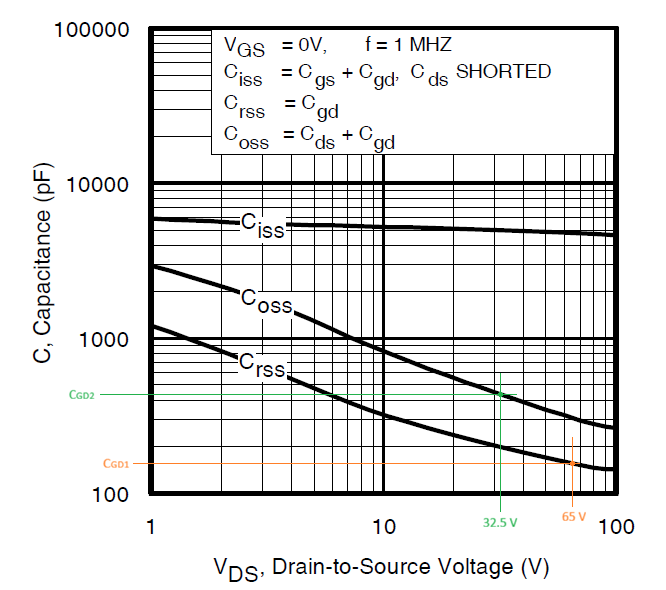
\includegraphics[width=0.8\linewidth]{CGD1_CGD2.png}
        \caption{Obtención de $C_{GD1}$ y $C_{GD2}$}
        \label{fig:CGD1_CGD2}
    \end{figure}

    Con los valores obtenidos en la Figura \ref{fig:CGD1_CGD2}, se obtienen los tiempos $t_{fu}$ y $t_{ru}$, que sirven para 
    el cálculo de las pérdidas energéticas (los cálculos se adjuntan en un documento de Excel). Obteniendo los siguientes resultados. 

    \begin{figure}[H]
        \centering
        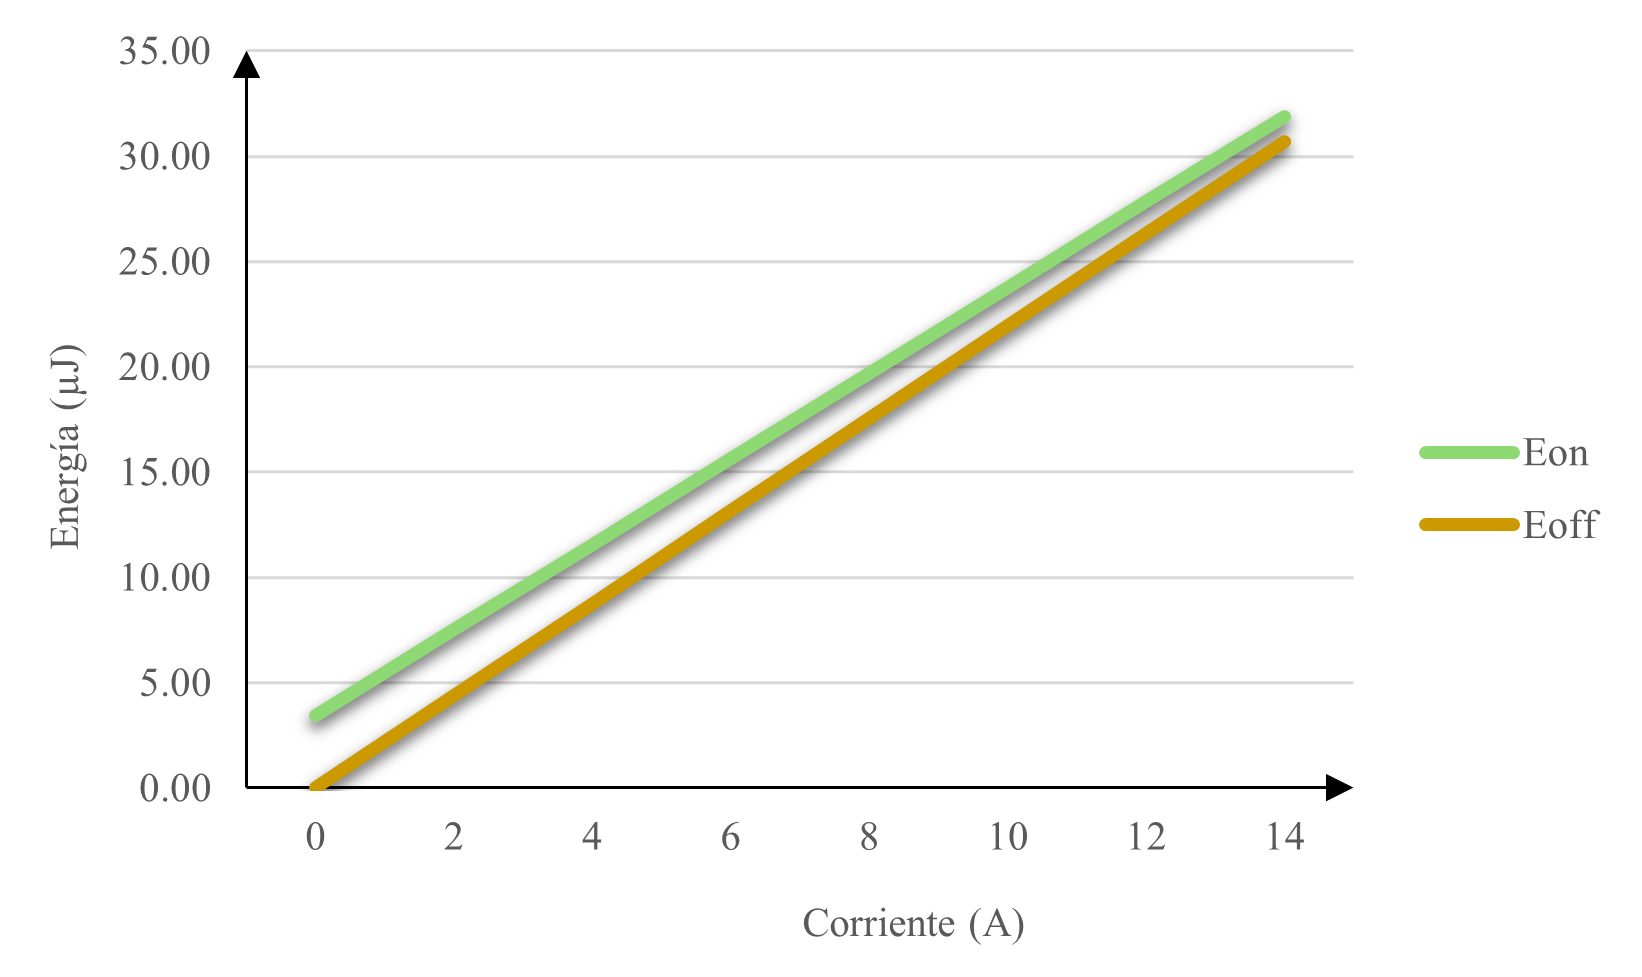
\includegraphics[width=0.8\linewidth]{Eon_Eoff_chart.png}
        \caption{Pérdidas de energía por conmutación del MOSFET}
        \label{fig:Eon_Eoff}
    \end{figure}

    Importante mencionar que estos cálculos se hacen en base a las condiciones de prueba del MOSFET mencionados en la hoja de datos, para
    la conformación del modelo térmico del dispositivo. Las pérdidas por conmutación en el convertidor Buck se analizarán posteriormente y
    se obtienen por medio de la siguiente ecuación \cite{InfineonMOSFETLosses2006}.

    \begin{equation}
        P_{sw} = (E_{on} + E_{off}) \cdot f_{sw} 
    \end{equation}












\subsection{Opciones para el diodo}

\begin{table}[H]
    \centering
    \renewcommand{\arraystretch}{1.5}
    \begin{tabularx}{\columnwidth}{
        >{\hsize=1.3\hsize\centering\arraybackslash}X 
        >{\hsize=1.1\hsize\centering\arraybackslash}X 
        >{\hsize=0.6\hsize\centering\arraybackslash}X 
        >{\hsize=0.6\hsize\centering\arraybackslash}X
    }
        \toprule
        Parámetro & HFA15PB60PbF & MUR1560 & 1N5408 \\
        \midrule
        $V_{RRM}$ [V] & 600 & 600 & 1000 \\
        $I_{F(AV)}$ [A] & 15 & 15 & 3 \\
        $V_F$ @ $I_F$ [V] & $\sim1.3$ @ 15A & $\sim1.2$ @ 15A & $\sim1.0$ @ 3A \\
        $t_{rr}$ [ns] & $\sim19$ & $\sim50$ & $>2000$ \\
        $Q_{rr}$ [nC] & $\sim80$ & $\sim150$ & N/A (very high) \\
        Tipo de recuperación & Ultrafast (soft) & Ultrafast & Standard (slow) \\
        $R_{\theta JC}$ [$^\circ$C/W] & $\sim2.0$ & $\sim2.5$ & $\sim3.0$ \\
        Aplicación típica & SMPS, converters & SMPS & Rectificación 50/60 Hz \\
        \bottomrule
    \end{tabularx}
    \caption{Comparación de diodos de potencia}
    \label{tab:diode_comparison}
\end{table}

El diodo seleccionado fue el HFA15PB60PbF debido a su bajo tiempo de recuperación inversa y baja carga de recuperación (Qrr), lo cual reduce significativamente las pérdidas de conmutación en aplicaciones de alta frecuencia como convertidores buck.

En comparación con diodos de propósito general como el 1N5408, el cual presenta tiempos de recuperación del orden de microsegundos, el HFA15PB60PbF ofrece tiempos en el orden de nanosegundos, haciéndolo adecuado para operación en alta frecuencia.

Asimismo, frente a otros diodos ultrarrápidos como el MUR1560, el HFA15PB60PbF presenta menor Qrr, lo que implica menores pérdidas de conmutación y menor generación de calor, siendo más eficiente para la aplicación propuesta.


\subsection{Modelado de pérdidas}
Para modelar las pérdidas del diodo (por conducción y conmutación), se extrajeron datos directamente de las curvas características del datasheet \cite{InfineonMOSFETLosses2006}. Posteriormente, se utilizaron líneas de tendencia (trendlines) para ajustar dichos datos a expresiones matemáticas, permitiendo obtener funciones continuas en lugar de valores discretos.

Este enfoque facilita una mejor aproximación del comportamiento real del dispositivo, ya que permite interpolar valores para diferentes condiciones de operación y reduce errores asociados al uso de puntos aislados. En el caso de las pérdidas por conmutación, se ajustó la relación entre la carga de recuperación inversa ($Q_{rr}$) y la razón de cambio de corriente ($di/dt$), mientras que para las pérdidas por conducción se modeló la característica $V$-$I$ del diodo mediante una aproximación lineal.

\begin{figure}[H]
        \centering
        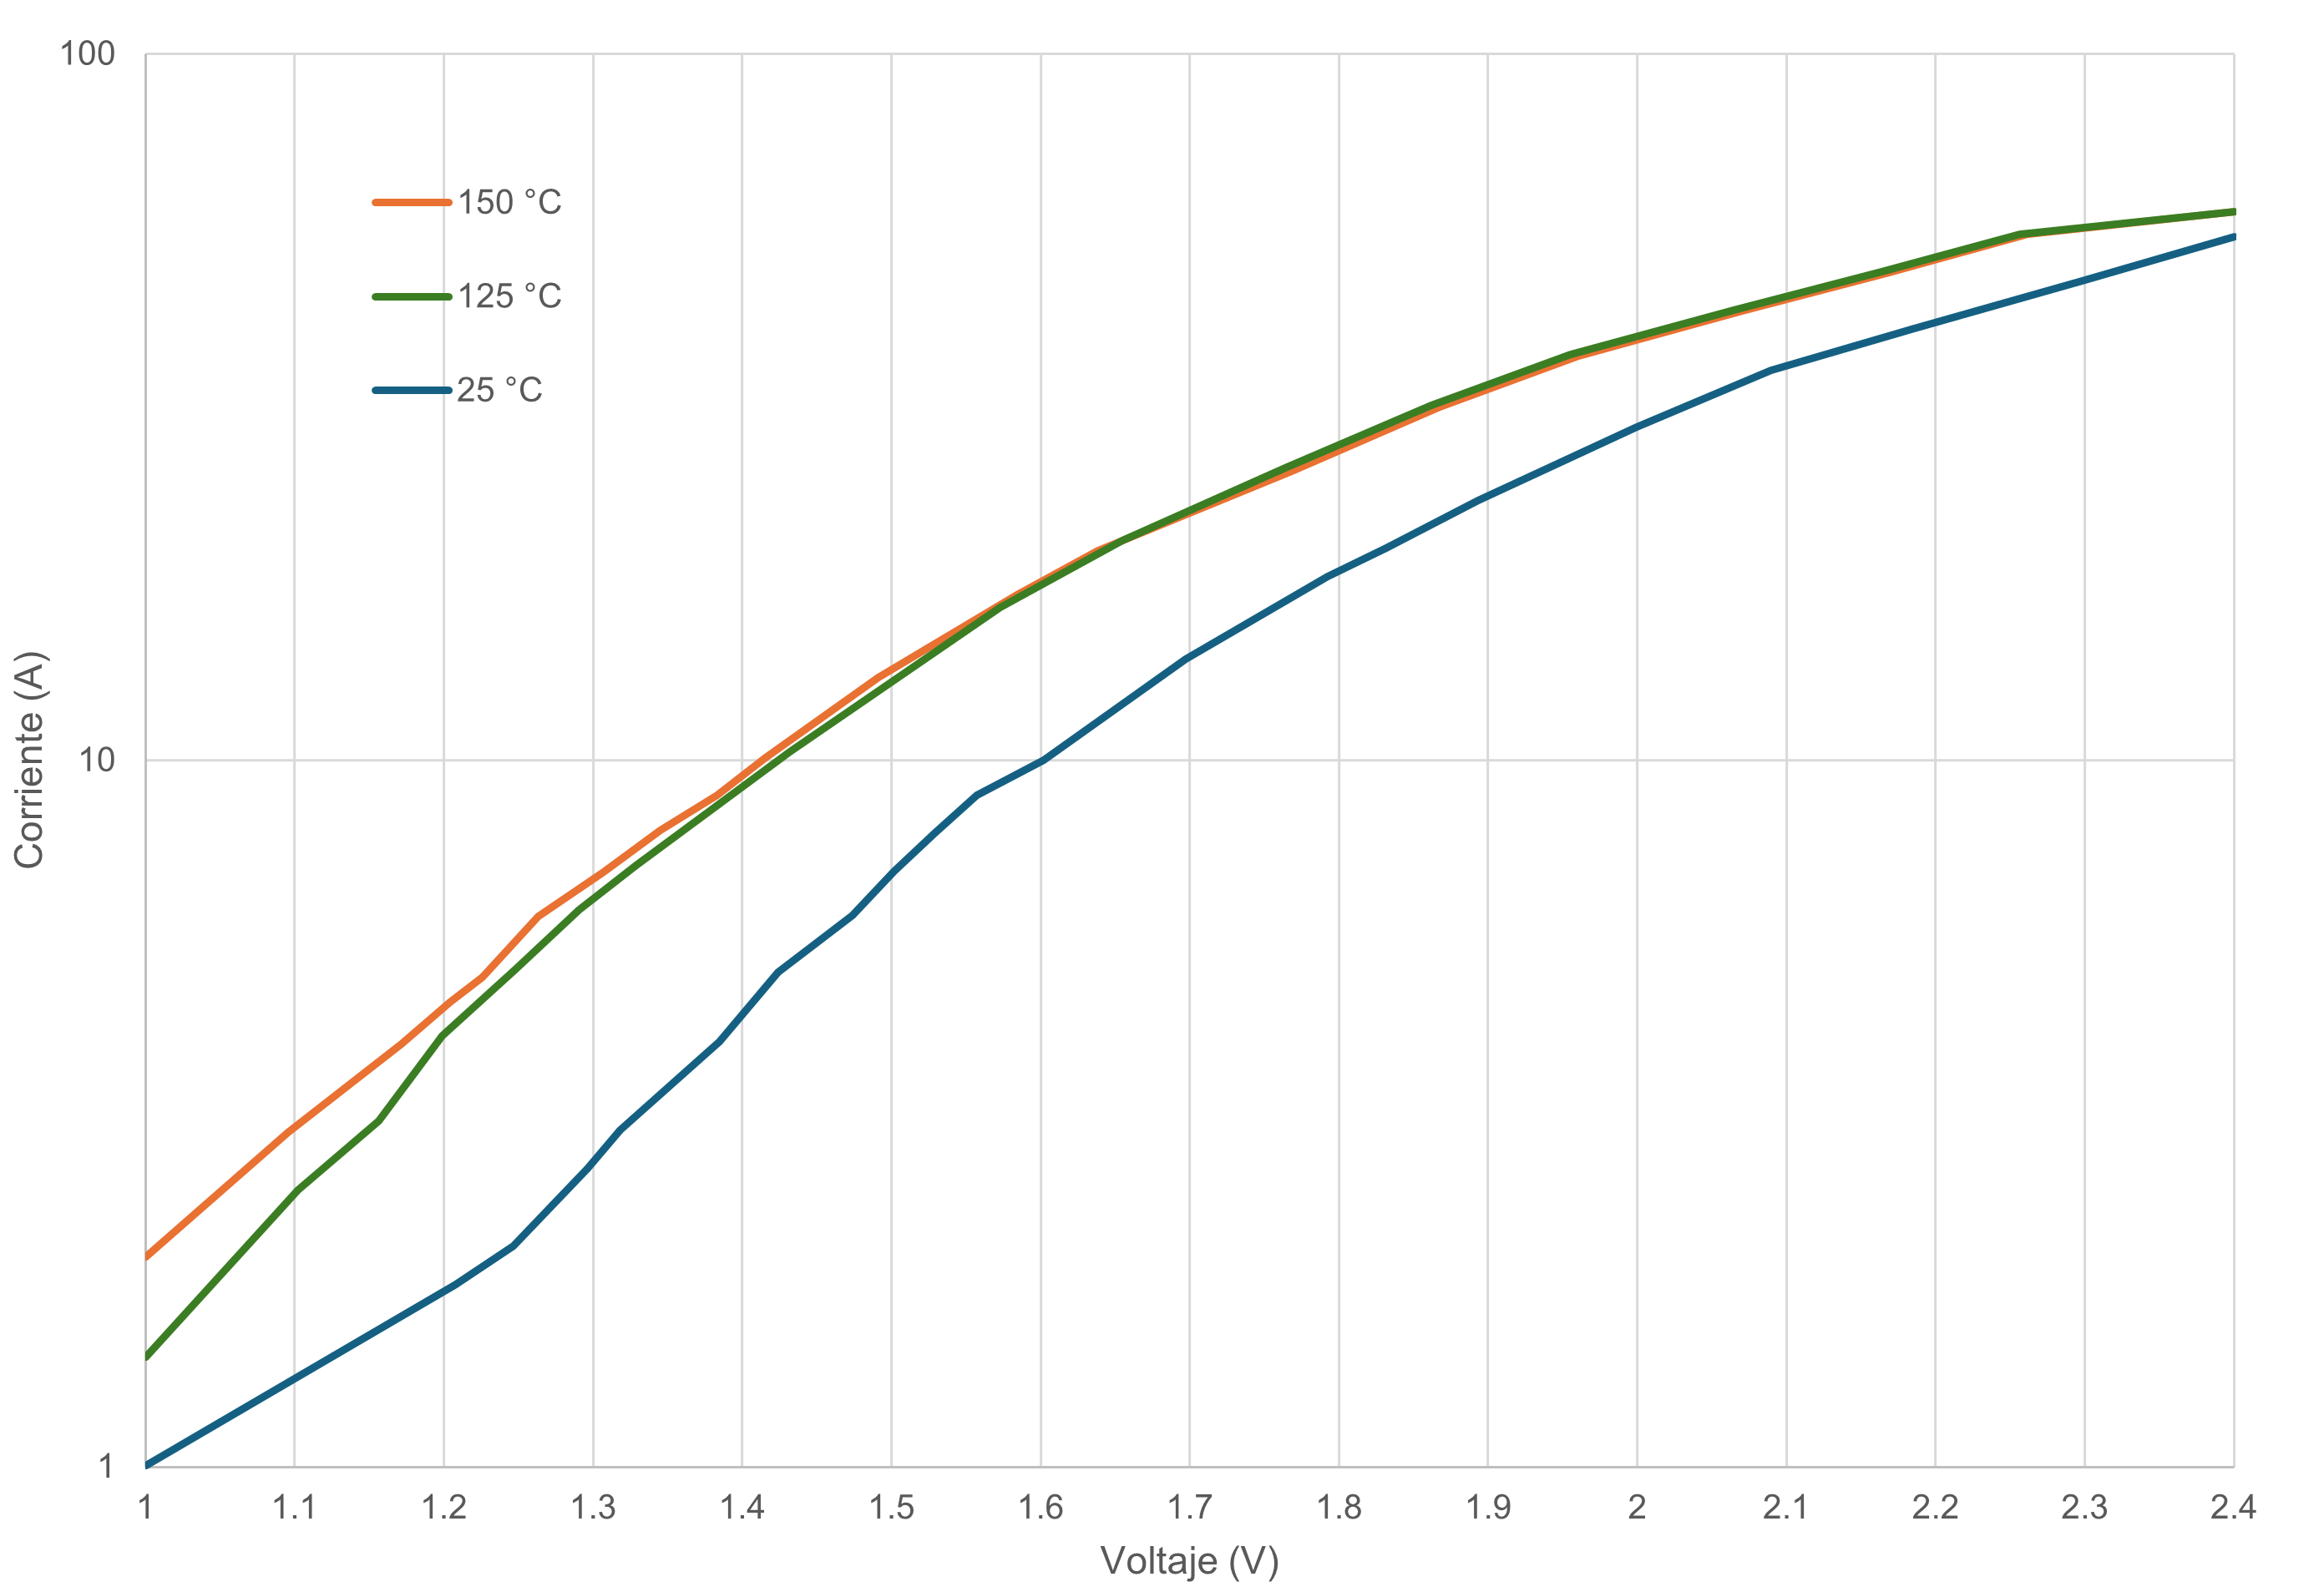
\includegraphics[width=0.8\linewidth]{CORRIENTEVOLLtaje.png}
        \caption{Curva de transferencia del diodo}
        \label{fig:DIODEtransfer}
    \end{figure}

\begin{figure}[H]
        \centering
        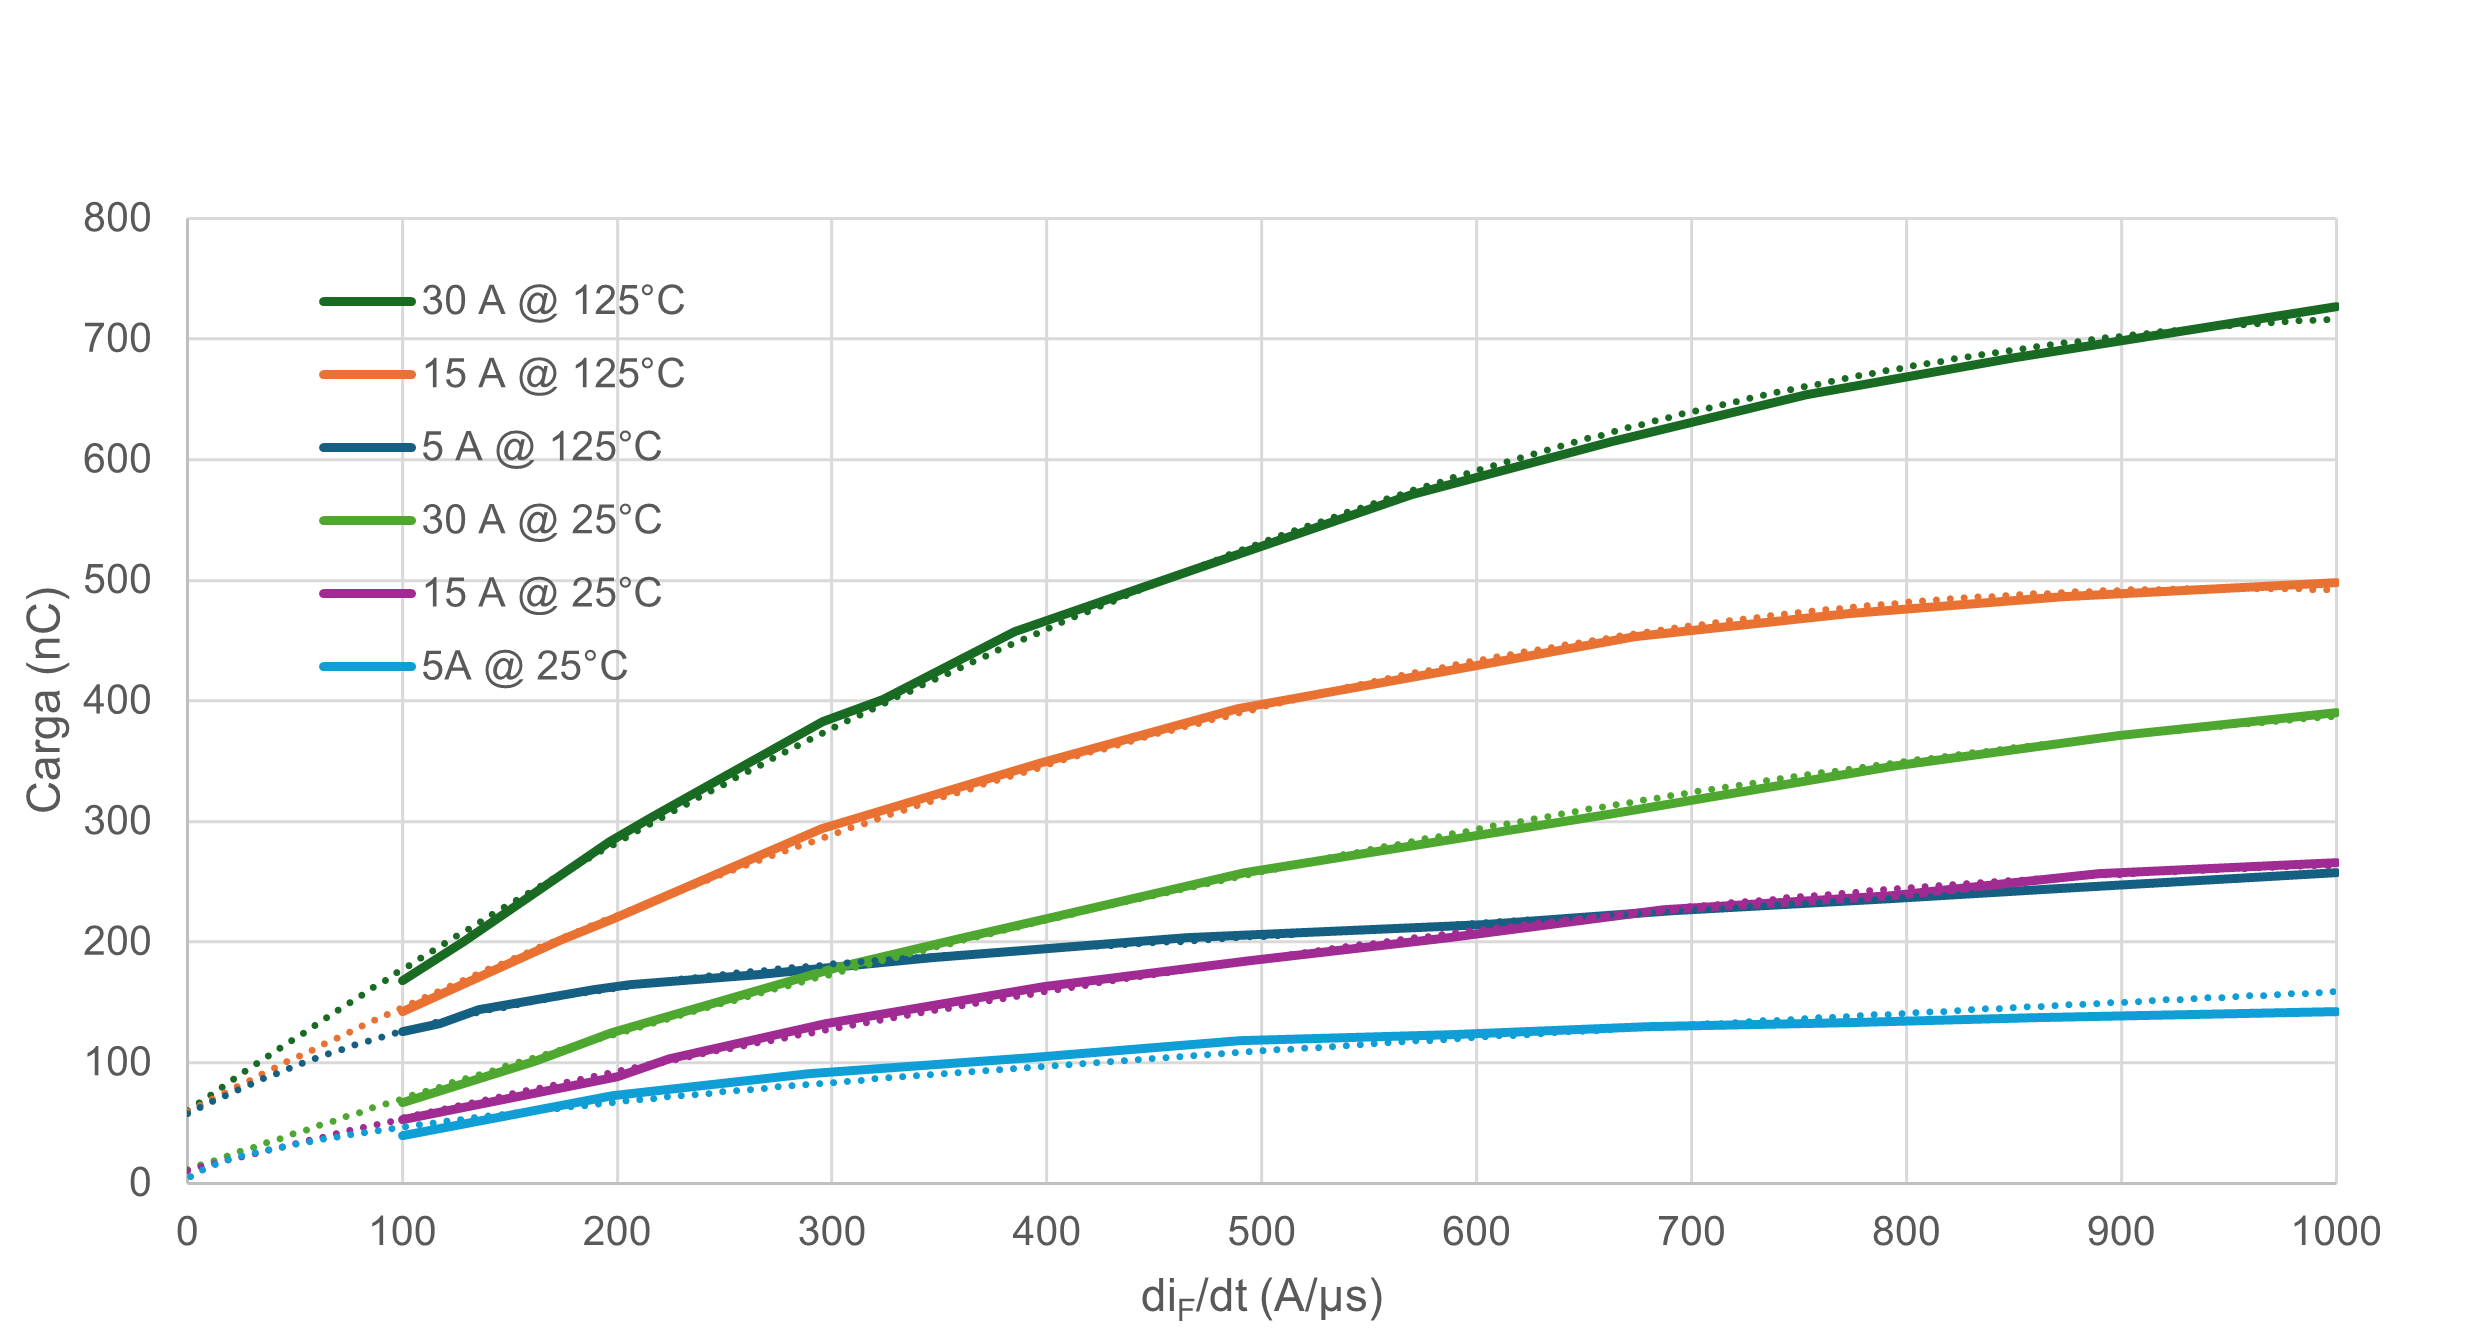
\includegraphics[width=0.8\linewidth]{qrr_didt.png}
        \caption{Carga de recuperación en reversa del diode como función de la tasa de cambio de la corriente directa del diodo}
        \label{fig:qrr25}
    \end{figure}



%%%%%%%%%%%%%%%%%%%%%%%%%%%%%%%%%%%%%%%%%%%%%%%%%%%%%%%%%%%%%%%%%%%%%%%%%%%%%%%%%%%%
%%%%%%%%%%%%%%%%%%%%%%%%%%%%%%%%%%%%%%%%%%%%%%%%%%%%%%%%%%%%%%%%%%%%%%%%%%%%%%%%%%%%
\section{Modelado térmico}

\subsection{Circuito térmico del sistema}

\subsection{Modelo Foster del MOSFET}

\subsection{Conversión a modelo Cauer del MOSFET}


%%%%%%%%%%%%%%%%%%%%%%%%%%%%%%%%%%%%%%%%%%%%%%%%%%%%%%%%%%%%%%%%%%%%%%%%%%%%%%%%%%%%
%%%%%%%%%%%%%%%%%%%%%%%%%%%%%%%%%%%%%%%%%%%%%%%%%%%%%%%%%%%%%%%%%%%%%%%%%%%%%%%%%%%%
\section{Validación térmica}

\subsection{Simulaciones térmicas}

\subsection{Cumplimiento de límites térmicos}



%%%%%%%%%%%%%%%%%%%%%%%%%%%%%%%%%%%%%%%%%%%%%%%%%%%%%%%%%%%%%%%%%%%%%%%%%%%%%%%%%%%%
%%%%%%%%%%%%%%%%%%%%%%%%%%%%%%%%%%%%%%%%%%%%%%%%%%%%%%%%%%%%%%%%%%%%%%%%%%%%%%%%%%%%
\section{Pérdidas y eficiencia}






%%%%%%%%%%%%%%%%%%%%%%%%%%%%%%%%%%%%%%%%%%%%%%%%%%%%%%%%%%%%%%%%%%%%%%%%%%%%%%%%%%%%
%%%%%%%%%%%%%%%%%%%%%%%%%%%%%%%%%%%%%%%%%%%%%%%%%%%%%%%%%%%%%%%%%%%%%%%%%%%%%%%%%%%%
\section{Conclusiones}
Las conclusiones van aquí.

%%%%%%%%%%%%%%%%%%%%%%%%%%%%%%%%%%%%%%%%%%%%%%%%%%%%%%%%%%%%%%%%%%%%%%%%%%%%%%%%%%%%
%%%%%%%%%%%%%%%%%%%%%%%%%%%%%%%%%%%%%%%%%%%%%%%%%%%%%%%%%%%%%%%%%%%%%%%%%%%%%%%%%%%%
\appendices
\section{Pendiente}
El texto relacionado al apéndice va aquí.


\printbibliography

%%%%%%%%%%%%%%%%%%%%%%%%%%%%%%%%%%%%%%%%%%%%%%%%%%%%%%%%%%%%%%%%%%%%%%%%%%%%%%%%%%%%
%%%%%%%%%%%%%%%%%%%%%%%%%%%%%%%%%%%%%%%%%%%%%%%%%%%%%%%%%%%%%%%%%%%%%%%%%%%%%%%%%%%%
\section{Biografías de los autores}



 
\begin{IEEEbiographynophoto}{Matías A. Camacho}
        Estudiante del Instituto Tecnológico de Costa Rica (TEC) en la carrera de ingeniería electrónica.
        
        Correo: jeacamacho@estudiantec.cr
\end{IEEEbiographynophoto}

\begin{IEEEbiographynophoto}{Juan P. Elizondo}
        Realizó sus estudios de secundaria en el SNCCCR, sede UNA Región Brunca, y actualmente cursa la carrera de Ingeniería Electrónica en el Instituto Tecnológico de Costa Rica (TEC). 
        
        Fue estudiante de la Universidad de Costa Rica (UCR) durante el año 2022 y participó en programas de estudio en matemática en la Universidad Nacional (UNA) durante los años 2020 y 2021. 
        
        Cuenta con preparación y/o experiencia en áreas como:
        \begin{itemize}
            \item Arquitectura básica de redes, CISCO CCNA V7 (ITN), (2021).
            \item Fundamentos de ciberseguridad, CISCO Systems, (2022).
            \item Programa de tutorías estudiantiles, Tecnológico de Costa Rica, (2024).
            \item Diseño de circuitos digitales, TEC (2025).
        \end{itemize}
        
        Correo: juelizondo@estudiantec.cr
\end{IEEEbiographynophoto}



\vfill

\end{document}






